\documentclass[9pt]{article}
\usepackage{fullpage}
\usepackage{amsmath}
\usepackage{amssymb}
\usepackage{graphics}
\usepackage[usenames]{color}
\usepackage{hyperref}
\usepackage{graphicx,wrapfig}
\usepackage{wallpaper}

\newcommand{\addphoto}[2]{%
  \smash{%
    \makebox[0pt][l]{%
      \raisebox{#1mm}{%
        \hspace{#2mm}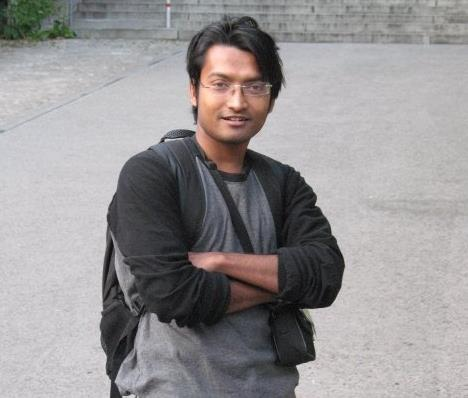
\includegraphics[scale=1]{mypic_1}%
      }%
     }%
  }%
}
\hypersetup{
    colorlinks=true,
    citecolor=blue,%
    filecolor=blue,%
    linkcolor=blue,%
    urlcolor=blue
}


\leftmargin=0.25in
\oddsidemargin=0.25in
\textwidth=6.0in
\topmargin=-0.25in
\textheight=9.25in
\newcommand{\p}{p{8cm}}

\raggedright

\pagenumbering{arabic}

\def\bull{\vrule height 0.8ex width .7ex depth -.1ex }
% DEFINITIONS FOR RESUME

\newenvironment{changemargin}[2]{%
  \begin{list}{}{%
    \setlength{\topsep}{0pt}%
    \setlength{\leftmargin}{#1}%
    \setlength{\rightmargin}{#2}%
    \setlength{\listparindent}{\parindent}%
    \setlength{\itemindent}{\parindent}%
    \setlength{\parsep}{\parskip}%
  }%
  \item[]}{\end{list}
}

\newcommand{\lineover}{
	\begin{changemargin}{-0.05in}{-0.05in}
		\vspace*{-8pt}
		\hrulefill \\
		\vspace*{-2pt}
	\end{changemargin}
}

\newcommand{\header}[1]{
	\begin{changemargin}{-0.5in}{-0.5in}
		\scshape{#1}\\
  	\lineover
	\end{changemargin}
}

\newcommand{\cmnt}[1]{}

\newcommand{\contact}[4]{
	\begin{changemargin}{-0.5in}{-0.5in}
		\begin{center}
			{\Large \scshape {#1}}\\ \smallskip
			{#2}\\ \smallskip 
			{#3}\\ \smallskip
			{#4}\smallskip
		\end{center}
	\end{changemargin}
}

\newenvironment{body} {
	\vspace*{-16pt}
	\begin{changemargin}{-0.25in}{-0.5in}
  }	
	{\end{changemargin}
}	

\newcommand{\school}[4]{
	\textbf{#1} \hfill \emph{#2\\}
	#3\\ 
	#4\\
}

% END RESUME DEFINITIONS

\begin{document}

%%%%%%%%%%%%%%%%%%%%%%%%%%%%%%%%%%%%%%%%%%%%%%%%%%%%%%%%%%%%%%%%%%%%%%%%%%%%%%%%
% Name
	\begin{changemargin}{-0.5in}{-0.5in}
\begin{tabular}{lr}
\begin{tabular}{c}
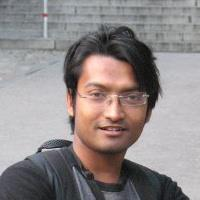
\includegraphics[height=35mm,width=35mm]{mypic3.png}
\end{tabular} & 
\begin{tabular}{c}
\\ \\  
\qquad\qquad\qquad\qquad\qquad\qquad\qquad {\Large Sandeep Dasgupta} \\ 
\qquad\qquad\qquad\qquad\qquad\qquad\qquad\ {\small{\underline{Email}: sdasgup3 [at] cs [dot] illinois [dot] edu}} \\
\qquad\qquad\qquad\qquad\qquad\qquad\qquad\quad\quad {\small{\underline{Url}: \url{http://web.engr.illinois.edu/~sdasgup3}}} \\
\qquad\qquad\qquad{\small{\underline{Mobile}: (+1) 2174172344}} \\
\end{tabular} \\
&\\
\end{tabular} 

	\end{changemargin}


%%%%%%%%%%%%%%%%%%%%%%%%%%%%%%%%%%%%%%%%%%%%%%%%%%%%%%%%%%%%%%%%%%%%%%%%%%%%%%%%
% Objective
\header{Research Interest}

\begin{body}
	\vspace{14pt}
		Program Analysis \& Verification \\
		Compiler Optimizations \\
		Parallel Computing \\
		Programming Language Design \& Implementation \\
		High performance computing \\
 		Automated software verification \& quality assurance.
\end{body}

\smallskip


%%%%%%%%%%%%%%%%%%%%%%%%%%%%%%%%%%%%%%%%%%%%%%%%%%%%%%%%%%%%%%%%%%%%%%%%%%%%%%%%
% Education
\header{Academics}

\begin{body}
	\vspace{14pt}
	\textbf{PhD Computer Science }{} \hfill \\
	\emph{\href{http://cs.illinois.edu/}{CS @ Illinois Urbana Champaign}}{} \\
	\begin{itemize} \itemsep -0pt
		\item Currently working with \href{http://llvm.org/}{ LLVM Group} led by Prof. \href{http://llvm.cs.uiuc.edu/~vadve/Home.html}{Vikram S. Adve}
	\end{itemize}
 \medskip
	\textbf{M.Tech Computer Science \& Engineering -- CPI 9.00/10.00}{} \hfill \emph{June 2011}{} \\
	\emph{\href{http://www.iitk.ac.in/}{Indian Institute Of Technology Kanpur}, Kanpur, India.}{} \\
	\begin{itemize} \itemsep -0pt
		\item Secured \textbf{rank $1$} in M. Tech 2009 Batch, IIT Kanpur.
	\end{itemize}
  \medskip
	\textbf{B.E. Computer Science \& Engineering -- \emph{First Class with Honours}, 85.625/100.00} \hfill \emph{June 2006} \\
	\emph{\href{http://www.becs.ac.in/}{Bengal Engineering \& Science University, Shibpur}}, West Bengal, India.\\
	\begin{itemize} \itemsep -0pt
		\item Awarded \textbf{University Gold Medal} for securing 1st Rank in BE, Computer Science \& Engineering, 2002 batch.
		\item Awarded \textbf{Best Student Award}, sponsored by \href{http://www.tcs.com}{Tata Consultancy Services}, for outstanding performance in BE, Computer Science \& Engineering, 2002 batch.
	\end{itemize}
\end{body}

\smallskip


%%%%%%%%%%%%%%%%%%%%%%%%%%%%%%%%%%%%%%%%%%%%%%%%%%%%%%%%%%%%%%%%%%%%%%%%%%%%%%%%
% MTech Thesis
\header{M.Tech Thesis \hfill Joint supervision of \href{http://www.cse.iitk.ac.in/users/karkare/}{Dr. Amey karkare} \& \href{http://www.cse.iitk.ac.in/users/ska/}{Dr.  Sanjeev K Aggarwal} }

\begin{body}
	\vspace{14pt}
	\textbf {\href{http://www.cse.iitk.ac.in/users/karkare/MTP/2010-11/sandeep2010precise.pdf}{Precise Shape Analysis Using Field Sensitivity}} \\
		\begin{itemize} \itemsep -0pt  
		\item[] To disambiguate heap allocated data-structures by estimating the shape (Tree, Dag or Cyclic Graph ) of the data structure 
			accessible from each heap directed pointer. This will help in automatic parallelization of sequential code having heap 
			intensive data structures. The work mainly focuses on devising a novel shape analysis technique. 
		\end{itemize}
\end{body}

\smallskip

% Publications
\header{Publications}
\begin{body}
\vspace{14pt}
\textbf{Papers in Conferences}\\
	\vspace*{-4pt}
	\begin{itemize} \itemsep -0pt
		\item Sandeep Dasgupta \& Amey Karkare.\href{https://dl.dropbox.com/u/86719354/sac\_2012.pdf}{``\textbf{Precise shape analysis using field sensitivity}''}, in \emph{Proceedings of the 27th Annual ACM Symposium on Applied Computing}, SAC 2012, pages 1300-1307, New York, USA. ACM. \href{http://dx.doi.org/10.1145/2245276.2231982}{doi: 10.1145/2231936.2231982}, isbn: 978-1-4503-0857-1. \\
		\item Barnali Basak, Sandeep Dasgupta \& Amey Karkare.\href{https://dl.dropbox.com/u/86719354/parco\_2011.pdf}{``\textbf{Heap Dependence Analysis for Sequential Programs}''}, \emph{International Conference on Parallel Computing} (ParCo 2011), Ghent, Belgium, August 30 - September 2, 2011. \\
		\begin{itemize} \itemsep -0pt
			\item Published in: Applications, Tools and Techniques on the Road to Exascale Computing, 22 volume of Advances in 
				Parallel Computing, chapter: Heap Dependence Analysis for Sequential Programs, pages 99--106. IOS Press, May 2012. 
				doi: \href{http://dx.doi.org/10.3233/978-1-61499-041-3-99}{10.3233/978-1-61499-041-3-99}, isbn: 978-1-61499-040-6.
		\end{itemize}
	\end{itemize}

\textbf{Posters}\\
	\vspace*{-4pt}
	\begin{itemize} \itemsep -0pt
		\item Poster \href{https://dl.dropbox.com/u/86719354/poster_APLAS2010.pdf}{``\textbf{Dependence Analysis for Parallelization 
		of Sequential Programs}''} got accepted at APLAS`10 (the 8th ASIAN Symposium on Programming Languages \& Systems).
	\end{itemize}

\textbf{Journals}\\
	\vspace{-4pt}
	\begin{itemize} \itemsep -0pt
		\item  Sandeep Dasgupta, Amey Karkare \& P.\ Vinay K.\ Reddy. \href{https://dl.dropbox.com/u/86719354/publication_isse.pdf}{``\textbf{Precise shape analysis using field sensitivity}.''}, in \emph{Innovations in Systems and Software Engineering (ISSE)}, a NASA journal.
                 doi: \href{http://www.springerlink.com/openurl.asp?genre=article&id=doi:10.1007/s11334-013-0198-7}{10.1007/s11334-013-0198-7} 
	\end{itemize}
\end{body}

%%%%%%%%%%%%%%%%%%%%%%%%%%%%%%%%%%%%%%%%%%%%%%%%%%%%%%%%%%%%%%%%%%%%%%%%%%%%%%%%
%Teaching Experience
\header{Teaching Experience}

\begin{body}
	\vspace{14pt}
	\textbf{Indian Institute of Technology, Kanpur},  \hfill \emph{August 2009 - 2011}\\
	\vspace*{-4pt}
	\begin{itemize} \itemsep -0pt  % reduce space between items
		\item \textbf{Tutor} for \href{http://www.cse.iitk.ac.in/teaching/courses/ESc101.html}{ESc 101: Fundamentals of Computing}: An undergraduate course.
			\begin{itemize}
				\item Responsible for weekly lecture class on C - programming language, supervision of programming laboratory and grading assignments and term examinations.
			\end{itemize}
		\item \textbf{Teaching Assistant} for \href{http://www.cse.iitk.ac.in/teaching/courses/CS335.html}{CS 335: Principles of Compiler Design}: An undergraduate course.
			\begin{itemize}
				\item Responsible for mentoring a student group on a course project of developing a simple compiler (using a subset of C-language constructs) demonstrating most of the phases of compiler design starting from Lexical \& Syntax analysis upto Intermediate code generation.
				\item Grading assignments and term examinations.
			\end{itemize}
		\item \textbf{Teaching Assistant} for \href{http://www.cse.iitk.ac.in/teaching/courses/CS355.html}{CS355: Programming Tools and Techniques}: An undergraduate course.
			\begin{itemize}
				\item Grading assignments related to Software management tools such as make; Programming tools such as Python, Perl; Document preparation systems such as tex; Tools for building programs like Lex and Yacc.
			\end{itemize}
	\end{itemize}
\end{body}

\smallskip

%%%%%%%%%%%%%%%%%%%%%%%%%%%%%%%%%%%%%%%%%%%%%%%%%%%%%%%%%%%%%%%%%%%%%%%%%%%%%%%%

%Professional Experience
\header{Professional Experience}

\begin{body}
	\vspace{14pt}
	\href{http://www.intel.in/content/www/in/en/homepage.html}{\textbf{Intel Technology India Pvt. Ltd.}}, \emph{Component Design Engineer} \hfill \emph{August 2011 - Present}\\
	\vspace*{-4pt}
	\begin{itemize} \itemsep -0pt  % reduce space between items
		\item Work on design automation problems related to formal equivalence verification (FEV) of hardware designs.
		\item Build flows and methodologies to provide solutions to formally verify leading next generation CPU designs.
	\end{itemize}

	\href{http://www.interrasystems.com/}{\textbf {Interra Systems India Pvt. Ltd.}}, \emph{Senior Member Of Technical Staff} \hfill \emph{August 2006 - July 2009}\\
	\vspace*{-4pt}
	\begin{itemize} \itemsep -0pt
		\item Developer of Interra's premiere front-end analyzer products - Cheetah (SystemVerilog) and MVV(Mixed Verilog Vhdl) and 
		provided support for several new constructs of System Verilog IEEE-1800-2005, fixed tool bugs, created applications and contributed in performance Improvement. 		
		\item Involved in a critical service project for \href{http://www.atrenta.com/}{Atrenta (I) Pvt. Ltd.} for the development of System Verilog features in Spyglass DFT.
	\end{itemize}
\end{body}

\smallskip

%%%%%%%%%%%%%%%%%%%%%%%%%%%%%%%%%%%%%%%%%%%%%%%%%%%%%%%%%%%%%%%%%%%%%%%%%%%%%%%%
% Awards and Honors
\header{Achievements/Distinctions}

\begin{body}
	\vspace{14pt}
	\begin{itemize} \itemsep -0pt  % reduce space between items
		\item Awarded \textbf{University Gold Medal} for securing 1st Rank in BE, Computer Science \& Engineering, 2002 batch.\\
		\item Awarded \textbf{Best Student Award}, sponsored by \href{http://www.tcs.com}{Tata Consultancy Services}, for outstanding performance in BE, Computer Science \& Engineering, 2002 batch. \\
		\item \textbf{Secured Rank $1$}, in M. Tech 2009 Batch, IIT Kanpur.
		\item \textbf{Secured All India Rank $145$} (99.64 percentile) in GATE 2009, an exam for admission in Graduate Study.
		\item \textbf{Ranked $356^{th}$} (among 1 Lakh+ students) in WB-JEE, 2002, an exam for admission in undergraduate study.
		\item Awarded \textbf{Interra Humming Bird Award} in recognition of \& appreciation for providing excellent support to \href{}{Atrenta (I) Pvt. Ltd.} in the project ``IEEE compliance for Spyglass'', awarded by \href{http://www.interrasystems.com/}{Interra Systems India Pvt. Ltd.} 
	\end{itemize} 
\end{body}

\smallskip



\end{document}


\cmnt{
%%%%%%%%%%%%%%%%%%%%%%%%%%%%%%%%%%%%%%%%%%%%%%%%%%%%%%%%%%%%%%%%%%%%%%%%%%%%%%%%
% MTech Course Projects
\header{M.Tech Course Projects}

\begin{body}
	\vspace{14pt}
	\textbf{\href{http://www.cse.iitk.ac.in/teaching/courses/CS738.html}{Advanced Compiler Optimizations}} \\
		\begin{itemize} \itemsep -0pt 
			\item[] To Extend the Generic Data Flow Analyzer GDFA (of gcc) to the data flow frameworks where data flow information can
				be represented using bit vectors but the frameworks are not bit vector frameworks because they are non-separable e.g.,
				faint variable analysis, possible undefined variable analysis, strongly live variable analysis.
		\end{itemize}

  		\medskip

	\textbf{\href{http://www.cse.iitk.ac.in/teaching/courses/CS633.html}{Parallel Computing}} \\
		\begin{itemize} \itemsep -0pt 
			\item[] To design a customized processor (using parallel processing concepts) for the application of document retrieval
				system. We developed a \href{https://github.com/sdasgup3/Parallel-Processor-Design}{superscalar processor (with  an issue rate of 2)} using verilog hdl, and an assembler for that processor using flex and bison.
		\end{itemize}
\end{body}

\smallskip
\newpage

%%%%%%%%%%%%%%%%%%%%%%%%%%%%%%%%%%%%%%%%%%%%%%%%%%%%%%%%%%%%%%%%%%%%%%%%%%%%%%%%
% BTech Course Projects
\header{B.Tech Project \hfill under supervision of \href{http://cse.iitkgp.ac.in/~pb}{Dr. Partha Bhowmick}}

\begin{body}
	\vspace{14pt}
	\textbf{\href{http://dl.dropbox.com/u/86719354/BE_project.pdf}{Affine Transformation of Digital Curves Using Chain Codes.}}  \\
		\begin{itemize} \itemsep -0pt  
		\item[]  Affine Transformation of Digital Curves Using Chain Codes. The problem statement is to rotate a digital image by a given angle.
		\end{itemize}
\end{body}

\smallskip
\smallskip

%%%%%%%%%%%%%%%%%%%%%%%%%%%%%%%%%%%%%%%%%%%%%%%%%%%%%%%%%%%%%%%%%%%%%%%%%%%%%%%%
% References
\header{References}
	\vspace{14pt}

\begin{body}
%\begin{table}[position specifier]
%\centering
\begin{tabular}{l|l}

& \\
	\begin{tabular}{\p}
		\href{http://www.cse.iitk.ac.in/users/karkare/}{Dr. Amey Karkare}, \\
		Assistant Professor, \\
		Department Of Computer Science \& Engineering, \\
		Indian Institute Of Technology Kanpur, India. \\
		Phone:	+91 512 259 7520 (Office) \\
		Email: karkare@gmail.com, karkare@cse.iitk.ac.in	
                Mobile: 919532689131
	\end{tabular} &
	\begin{tabular}{\p}
		\href{http://cse.iitkgp.ac.in/~pb/}{Dr. Partha Bhowmick}, \\
		Professor, \\
		Department Of Computer Science \& Engineering, \\
		Indian Institute Of Technology Kharagpur, India. \\
		Phone:	+91-3222-283468 \\
		FAX:	+91-3222-278985 \\
		Email:	pb@cse.iitkgp.ernet.in \\
		gmail:	 bhowmick@gmail.com \\
	\end{tabular} \\
& \\ \hline
& \\
	\begin{tabular}{\p}
		\href{http://www.becs.ac.in/aboutjaya-sil-cstmenuitem}{Dr. Jaya Sil}, \\
		Professor, \\
		Department of Computer Science and Technology, \\
		Bengal Engineering \& Science University, Shibpure, West Bengal, India. \\
		Phone: +91 - 33 - 26684561/62/63 Ext. \\
		Email:	js@cs.becs.ac.in \\
		%Mobile: 09433283641 
	\end{tabular} &
	\begin{tabular}{\p}
	\href{http://www.linkedin.com/pub/neelu-bajaj/8/491/7a7}{Neelu Bajaj}, \\
	Director Engg. at Atrenta India Pvt. Ltd. \\
	Email: neelu@noida.atrenta.com \\
%	Mobile: (91) 9810803073.
	\end{tabular} \\ 
& \\ \hline
& \\
	\begin{tabular}{\p}
		\href{http://www.linkedin.com/pub/kausik-datta/1/9a8/964}{Kausik Datta}, \\
		Senior Manager at Mentor Graphics, \\
		Kolkata Area, India \\
		%Phone: +91 - 9830252538 \\
		Email:	datta.kausik@gmail.com \\
		%Mobile: 09433283641 
	\end{tabular} &
	\begin{tabular}{\p}
		\href{http://www.jaduniv.edu.in/profile.php?uid=615}{Dr. Samiran Chattopadhyay}, \\
		Head Of The Department, \\ 
		\href{http://www.jaduniv.edu.in/view\_department.php?deptid=90}{Department of Information Technology}, \href{http://www.jaduniv.edu.in/}{Jadavpur University}, \\
		West Bengal, India. \\
		PH: 2335-8321 (O), 2414-6666 \\
		Email:	samirancju@gmail.com \\
		Mobile: 91 9830613450
	\end{tabular} \\
& \\ \hline

\end{tabular}
	
\end{body}
}
